\documentclass[12pt,a4paper]{article}
\usepackage[utf8]{inputenc}
\usepackage{amsmath,amssymb,amsfonts,amsthm}
\usepackage{geometry}
\usepackage{fancyhdr}
\usepackage{lastpage}
\usepackage{graphicx}
\usepackage{enumitem}

% Page layout
\geometry{margin=1in}
\pagestyle{fancy}
\fancyhf{}
\lhead{Lucas Cassin Cruz Burke}
\rhead{AMATH 569}
\rfoot{Page \thepage\ of \pageref{LastPage}}

% Theorem environments
\theoremstyle{definition}
\newtheorem{problem}{Problem}
\theoremstyle{remark}
\newtheorem*{solution}{Solution}

\title{AMATH 569 Homework 6}
\author{Lucas Cassin Cruz Burke}
\date{May 31, 2023}

\begin{document}

\maketitle

% Problem 1
\begin{problem}
    Consider the sound waves generated by $$\psi_{tt} = c^2 \nabla^2 \psi, \qquad \nabla^2 = \frac{1}{r} \partial_r (r \partial_r) + \frac{1}{r^2}\partial_\theta^2 + \partial_z^2$$
    in a circular cylinder of radius $a$ and length $L$, where $\psi = 0$ at $r=a$ and $\psi=0$ at $z=0, L$. 

    Assume that the sound produced in this tube is symmetric, i.e. no $\theta$ dependence. Find the lowest three frequencies. Take $c=300$m/s, $a = 1$cm, $L =0.5$m. 
\end{problem}
\begin{solution}
    Since our domain is symmetric, we can drop the $\theta$ component of the Laplacian and write $$\nabla^2 = \frac{1}{r}\partial_r (r \partial_r) + \partial_z^2$$

    Our equation is then $$\psi_{tt} = c^2 \left[ \frac{1}{r}\partial_r (r \psi_r) + \psi_{zz} \right]$$

    We assume a separable solution of the form $\psi(r, z, t) = R(r) Z(z) T(t)$. Plugging this in and diving by $c^2 \psi$ gives us the equation $$\frac{T''}{c^2T} =  \frac{(rR')'}{rR} + \frac{Z''}{Z} = -k^2$$
    
    where $-k^2$ is a separation constant. For the $T$ dependence, we have $$T'' = -c^2 k^2 T \quad \Rightarrow \quad T = A \cos (ck t) + B \sin (ckt)$$

    For $R$ and $Z$, we note that the LHS is the sum of two constants, and so we separate our equation once more into the equations $$(rR')' = rR'' + R' = -\alpha^2 rR \quad \text{ and } \quad Z'' = -\beta^2 Z$$

    where $\alpha^2 + \beta^2 = k^2$. For $Z$ we have solutions $Z(z) = C \cos(\beta z) + D \sin (\beta z)$, while for the $R$ function, we can multiply by $r$ to get the order 0 Bessel equation $$r^2 R'' + rR' + \alpha^2 r^2 R = 0$$

    whose solution is given by the Bessel function of the first kind $R(r) = J_0(\alpha r)$.

    We can apply our boundary conditions for $r$ and $z$ to find acceptable values for $\alpha$ and $\beta$. We need $Z(0) = Z(l) = 0$, hence we must have $Z = A \sin (\frac{n \pi z}{L})$ for $n \in \{1, 2, \dots\}$. We also need $R(a) = 0$, hence we must have $R(r) = J_0(\frac{j_{0,m} r}{a})$, where $j_{0,m}$, $m \in \{1, 2, \dots\}$ is the $m$th root of $J_0$. 

    By our separation process, we must have $\alpha^2 + \beta^2 = k^2$, hence our $k$ values must satisfy $$k^2 = \frac{n^2 \pi^2}{L^2} + \frac{j_{0,m}^2}{a^2} = [4 \pi^2 n^2 + 10^6 j_{0,m}^2] [\frac{1}{\text{m}^2}]$$

    We see that energy jump to the second lowest radial mode is much greater than the corresponding jump for the lengthwise mode. Hence our lowest $k$ values will correspond to $m = 1$ and $n=1, 2, 3, 4$. The corresponding $k$ values are then given by 

    \begin{align*}
        k_1 &= \sqrt{4 \pi^2 + 10^6 j_{0,1}^2} [\frac{1}{\text{m}}] \approx 2404.80 [1/\text{m}]  \\
        k_2 &= \sqrt{16 \pi^2 + 10^6 j_{0,1}^2} [\frac{1}{\text{m}}] \approx 2404.83 [1/\text{m}] \\
        k_3 &= \sqrt{36 \pi^2 + 10^6 j_{0,1}^2} [\frac{1}{\text{m}}] \approx 2404.87 [1/\text{m}] \\
        k_4 &= \sqrt{64 \pi^2 + 10^6 j_{0,1}^2} [\frac{1}{\text{m}}] \approx 2404.93 [1/\text{m}] \\
    \end{align*}

    Hence our lowest frequences, given by $\frac{ck_n}{2\pi} = \frac{300 [\text{m/s}]\times k_n}{2 \pi} [1/\text{s}]$, are $$f_1 = 114820 \text{ Hz} \qquad f_2 =  114822 \text{ Hz} \qquad f_3 = 114824 \text{ Hz} \qquad f_4 =  114827 \text{ Hz}$$
\end{solution}

% Problem 2
\begin{problem}
    Consider the wave function $\psi$ for an electron of mass $\mu$ in a sphere surrounded by an infinite potential at a radius $a$ from the nucleus, which just means that $\psi = 0$ at $r=a$. $$i \hbar \psi_t = -\frac{\hbar^2}{2\mu} \nabla^2 \psi$$
    Find the energy levels for the symmetric case, where $\psi$ does not depend on $\theta$ and $\phi$. Your answer should be exact and in terms of parameters given. 
\end{problem}
\begin{solution}
    We assume a separable solution $\psi(r, t) = R(t) T(t)$. Then, using the spherical Laplacian, we have

    $$i \hbar RT_t = - \frac{\hbar^2}{2\mu r}(rR)_{rr}T \qquad \Rightarrow \qquad i \hbar \frac{T'}{T} = - \frac{\hbar^2}{2\mu} \frac{(rR)''}{rR} = E$$

    where $E$ is a separation constant. For the $t$ dependence we have $$T' = \frac{-i E}{\hbar} T \qquad \Rightarrow \qquad T(t) = A e^{- i E t/\hbar}$$

    For the $r$ dependence we have $$ rR'' + 2R'  + \frac{2 \mu E}{\hbar^2}rR = 0$$

    Multiplying by $r$ gives us the first order spherical Bessel equation $$r^2 R'' + 2rR' + \frac{2 \mu E}{\hbar^2} r^2R = 0$$

    whose solution is given by the spherical Bessel function $$R(r) = B j_0\left(\frac{\sqrt{2\mu E}}{\hbar} r\right) + C y_0 \left(\frac{\sqrt{2\mu E}}{\hbar} r\right)$$

    where $j_0$ and $y_0$ are the spherical Bessel functions of the first and second kind, respectively. Since we require that $R$ is finite at $r =0$, we must have $C = 0$. Furthermore, the boundary condition $\psi(a) = 0$ implies that $R(a) = 0$, hence we have $$R(a) = B j_0 \left(\frac{\sqrt{2\mu E}}{\hbar} a\right) = 0 \qquad \Rightarrow \qquad \frac{\sqrt{2\mu E}}{\hbar} a = \lambda_n $$

    where $\lambda_n$ is the $n$ root of the spherical Bessel function $j_0$. Hence, our energy levels are given by $$E_n = \frac{\hbar^2 \lambda_n^2}{2 \mu a^2} \qquad n \in \{1, 2, \dots \}$$

    where $\lambda_n$ are the zeros of the spherical Bessel function. 

    
\end{solution}

% Problem 3
\begin{problem}
    Consider the Legendre equation $$\frac{d}{dx} \left[ (1-x^2) \frac{d}{dx}y(x) \right] + n(n+1)y(x)=0, \quad -1 \le x \le 1,$$
    with the condition that $y(\pm 1)$ are bounded. The solutions are the Legendre polynomials $P_n(x)$, which are given by the Rodrigue's formula $$P_n(x) = \frac{1}{2^nn!} \frac{d^n}{dx^n} (x^2 - 1)^n$$

    For example, $P_2(x) = \frac{1}{2} (3x^2-1)$. 

    Compute the first four coefficients in the Legendre expansion 
    
    $$f(x) = \sum_{n=0}^\infty a_n P_n(x), \qquad \text{where } a_n = \frac{2n+1}{2} \int_{-1}^1 f(x) P_n(x) dx \quad \text{ for } f(x) = \begin{cases} 0 & \text{for $-1 < x < 0$} \\ x & \text{for $0 < x < 1$}\end{cases}$$

    Plot the approximation of the sum consisting of one, two, three and four terms along with the original function $f(x)$. 
\end{problem}
\begin{solution}
    Let's begin by writing out the first four Legendre polynomials explicitely. We have \begin{align*}
        P_0(x) &= 1 \\
        P_1(x) &= \frac{1}{2} \frac{d}{dx} (x^2-1) = x\\
        P_2(x) &= \frac{1}{8} \frac{d^2}{dx^2} (x^2-1)^2 = \frac{1}{2}(3x^2-1) \\
        P_3(x) &= \frac{1}{48} \frac{d^3}{dx^3} (x^2-1)^3 = \frac{1}{2} (5x^3 - 3x)
    \end{align*}

    Using these, we can compute the coefficients $a_0, a_1, a_2, a_3$ using the above formula for $f(x)$. Starting with $a_0$, we have

    \begin{align*}
        a_0 &= \frac{1}{2} \int_{-1}^1 f(x) P_0(x) dx = \frac{1}{2} \int_{0}^1 x dx = \frac{1}{4} x^2 \Bigg|_{0}^1 = \frac{1}{4} \\
        a_1 &= \frac{3}{2} \int_{-1}^1 f(x) P_1(x) = \frac{3}{2} \int_0^1 x^2 dx = \frac{3}{6} x^3 \Bigg|_0^1 = \frac{1}{2} \\
        a_2 &= \frac{5}{2} \int_{-1}^1 f(x) P_2(x) dx = \frac{5}{4} \int_0^1 (3x^3 - x) dx = \frac{5}{4} \left(\frac{3}{4} x^4 - \frac{1}{2} x^2\right) \Bigg|_0^1 = \frac{5}{16} \\
        a_3 &= \frac{7}{2} \int_{-1}^1 f(x) P_2(x) dx = \frac{7}{4} \int_0^1 (5x^4 - 3x^2) dx = \frac{7}{4} \left( x^5 - x^3 \right) \Bigg|_0^1 = 0
    \end{align*}

    Hence our fourth order Legendre expansion approximation for $f(x)$ is given by $$f(x) \approx \frac{1}{4} P_0(x) + \frac{1}{2} P_1(x) + \frac{5}{16} P_2(x) + 0 \cdot P_3(x) = \frac{1}{4} + \frac{x}{2} + \frac{5}{32} (3x^2-1)$$ 

    The $f(x)$ function along with the first four Legendre approximations are plotted below.

    \begin{figure}[h!]
        \centering
        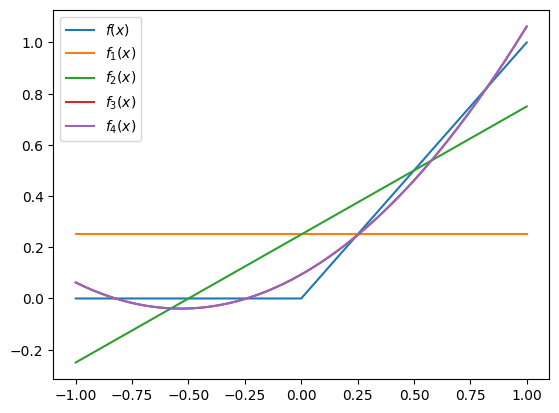
\includegraphics{Legendre.png}
        \caption{The function $f(x)$ along with its first four Legendre approximations.}
    \end{figure}

\end{solution}

\end{document}
